\documentclass[12pt,twoside]{report}
\pagenumbering{roman}

\usepackage{graphicx}
\usepackage{subcaption}

\usepackage[utf8]{inputenc}
\usepackage[german]{babel}

% \degree{} command
\usepackage{gensymb}

\usepackage{hyperref}
\hypersetup{
  colorlinks=true,
  linkcolor=blue,
  filecolor=magenta,      
  urlcolor=cyan,
}

\urlstyle{same}

% CONSTANTS BEGIN
\newcommand{\github_repo}{\href{https://github.com/Pierrefha/ees-buggy-project}{GitHub-Repository}}
\newcommand{\referenz_code}{\href{https://github.com/tomfclarke/adafruit-motor-hat-cpp-library}{Referenz-Code}}

\begin{document}
\begin{titlepage}
    \begin{center}
        \vspace*{1cm}
            
        \Huge
        \textbf{Lernportfolio}

        \vspace{1.5cm}
            
        \normalsize
        \textbf{Pierre Dahmani pd1528s TODO MATRIKEL\\
        Jens Peter jd8389s TODO Matrikel\\
        Leonhard Kipp lk2149s 3188047\\}
            
        \vfill
            
        EES Buggy-Projekt 
        \vspace{0.8cm}
            
        %% TODO Add title pic
        %% \includegraphics[width=0.4\textwidth]{university}
        \pagebreak
    \end{center}
\end{titlepage}

% TODO Inhaltsverzeichnis

\section{Aufbau des Buggy}

\begin{figure}[h!]
  \centering
  \captionsetup[subfigure]{labelformat=empty}
  \begin{subfigure}{0.45\linewidth}
    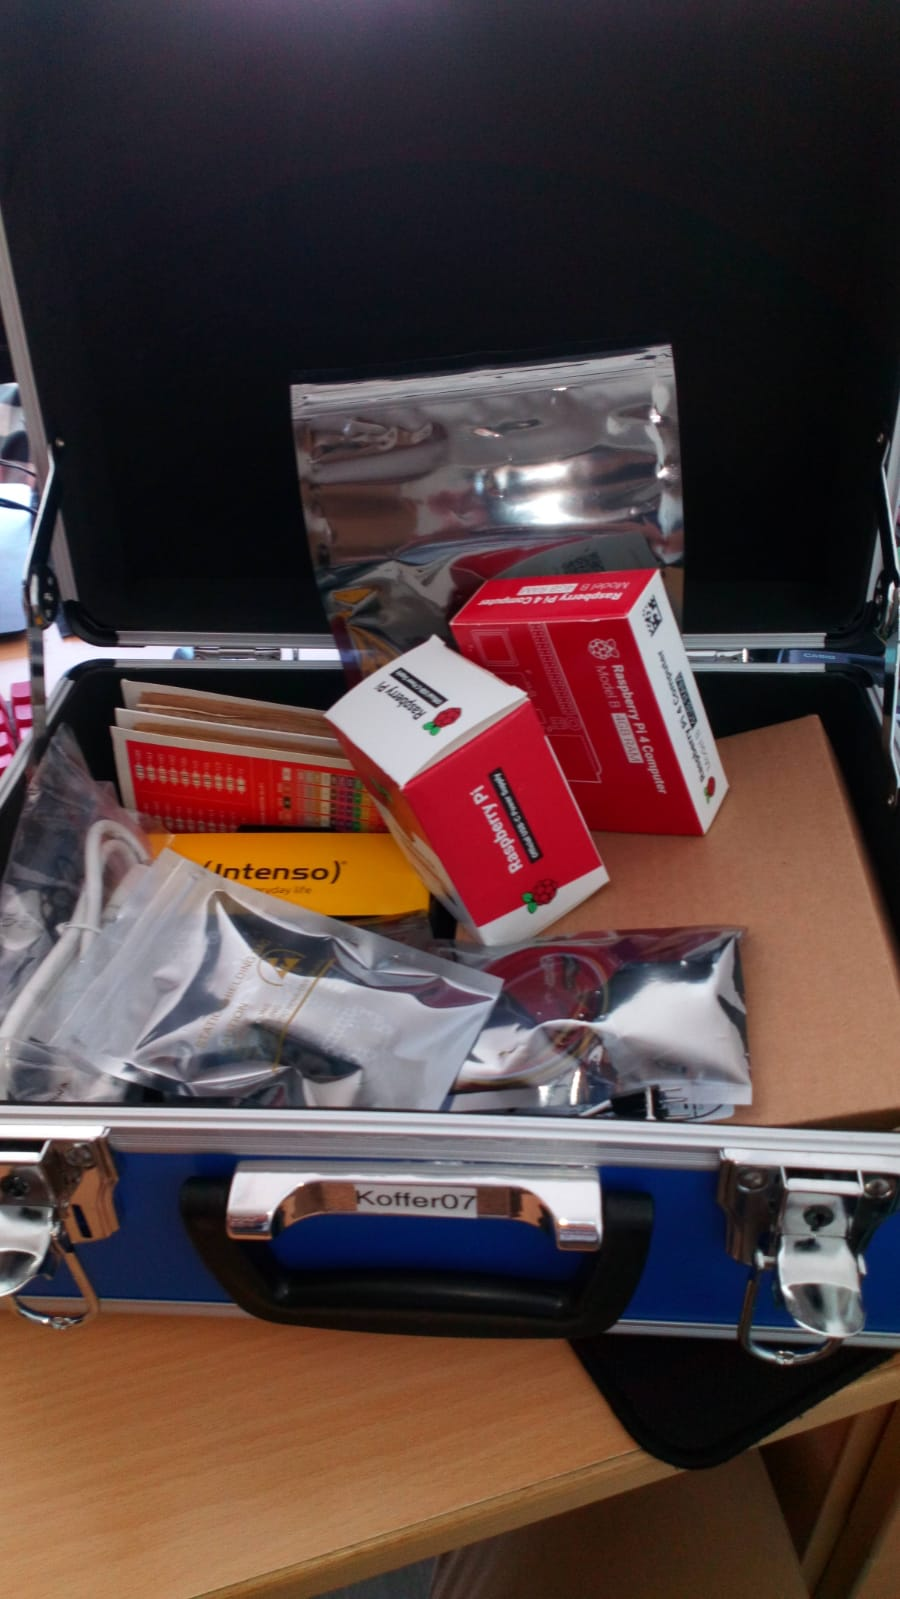
\includegraphics[width=\linewidth]{lernportfolio_assets/Buggy_Koffer.jpeg}
    \caption{Der Buggy vor dem Aufbau.}
  \end{subfigure}
  \begin{subfigure}{0.45\linewidth}
    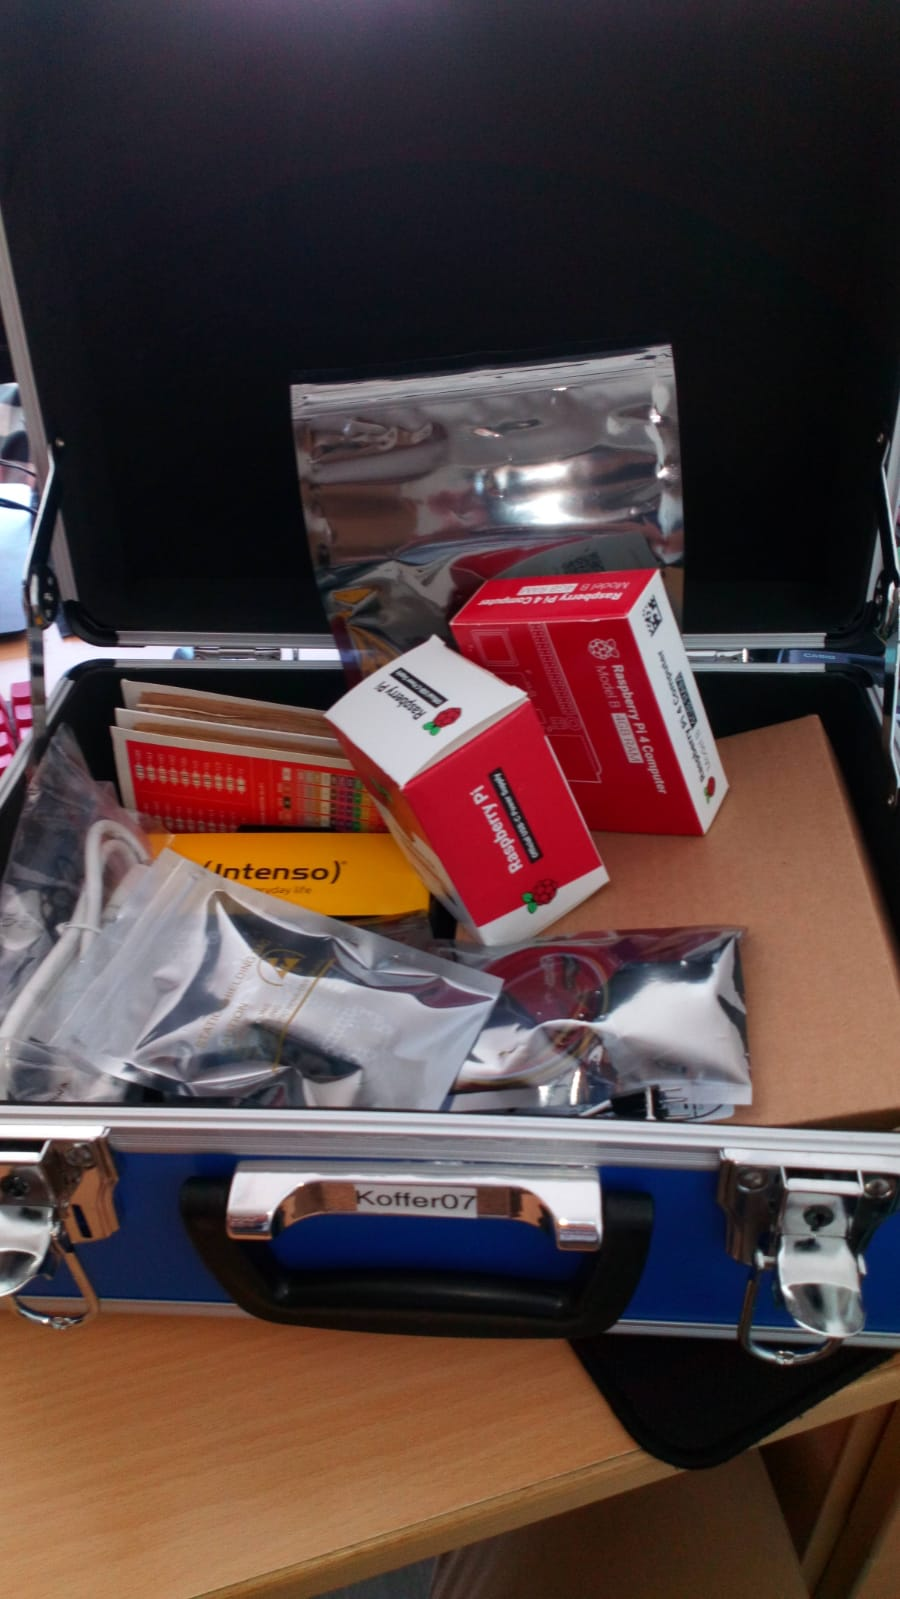
\includegraphics[width=\linewidth]{lernportfolio_assets/Buggy_Koffer.jpeg}
    \caption{Und danach.}
  \end{subfigure}
\end{figure}

Der Buggy wurde vor der Herausgabe des Arbeitsauftrages zusammengebaut. Zwischenschritte sind daher nicht bildlich festgehalten. 

Der Zusammenbau des Buggies verlief problemlos. Der Text ist insgesamt verständlich geschrieben und war eine große Unterstützung.

% Wollen wir das aufnehmen?
% Im Text ist der Genetiv von ``der Buggy'' durchgehend ``des Buggies''. Mit Verweis
% auf \url{https://www.duden.de/rechtschreibung/Buggy} ist der korrekte - und
% kontraintuitive - Genetiv ``des Buggys''.
In den meisten Bildern (außer auf Seite IV) ist der Buggy mit roter Platte gezeigt, wenngleich die Anleitung hier den weißen Winkel vorsieht. Eine Anmerkung, dass der Buggy im Folgendem mit roter Platte statt Winkel gezeigt wird, hätte eine kurze Verwirrung meinerseits verhindert.

Als Ubuntu-Nutzer muss man keine zusätzliche Software installieren um eine SSH-Verbindung herzustellen. Eine Ergänzung, dass \href{https://invisible-island.net/xterm/}{XTerm} eine Empfehlung an die Windows-Nutzer ist, wäre daher angebracht. Bei dieser Bemerkung wird davon ausgegangen, dass mit XTerm an dieser Stelle \href{https://mobaxterm.mobatek.net/}{MobaXterm} gemeint ist und nicht der Terminal Emulator XTerm. 

Für den kompletten Zusammenbau wurden insgesamt 1 Stunden benötigt. Die meiste Zeit nahm die SSH-Verbindung in Anspruch.

% TODO 1.4



\section{Motorensteuerung}

Videos zu den Tests der Motorensteuerung sind unter: TODO LINK EINFÜGEN
Der Quelltext kann unter \github_repo{} eingesehen werden.

Herausforderungen bei der Programmierung waren vor allem 3 Punkte: 1. Finden der wichtigen
Dokumentation, 2. Verstehen der Dokumentation und 3. Extraktion der relevanten
Informationen.
Durch die Schematas unter
\url{https://learn.adafruit.com/adafruit-dc-and-stepper-motor-hat-for-raspberry-pi/downloads}
konnte die Verknüpfung der GPIO's des Raspberry Pi's mit dem Motorhat entnommen
werden. Durch die Datenblätter wurde die Funktionsweise des '\referenz-code's
verständlich.
In den ersten Testläufen hat sich der Buggy beim Forwärtsfahren im Kreis
gedreht. Die Motoren haben in unterschiedliche Richtungen gedreht. Dieses
Verhalten war verständlich, da beide Motoren auf forwärts gestellt waren, was
synonym für eine rechtsläufige Bewegung war. Für das rechte Rad bedeutet
'rechtsläufig' forwärts. Für das linke Rad, welches durch den Anbau 
180\degree{} um die Z-Achse gedreht ist, bedeutet dies rückwärts.
Das Problem konnte behoben werden, indem die beiden Pins, welche für die Richtung
zuständig sind, vertauscht wurden. So wurde jede rechtsläufige Bewegung zu einer
linksläufigen und vice versa. Ein Forwärts-Kommando an das linke Rad wurde nun
korrekterweise automatisch in eine linksläufige Bewegung übersetzt.
Weiterhin war es ein Problem den Buggy konsistent losfahren zu lassen. Niedrige 
Geschwindigkeit sind beim Start zu gering, um die Motoren drehen zu
lassen. Das hat dazu geführt, dass der Buggy oft nicht losfuhr, trotz eines
forwärts Kommandos. Dieses Problem konnte behoben werden, indem eine Mindestgeschwindigkeit
eingestellt worden ist, sodass der Buggy nicht mit niedrigen Geschwindigkeiten
konfigurierbar ist.

Neben den technischen Herausforderungen war auch das Testen des Codes auf dem
Raspberry Pi eine Umgewöhnung. Der Code konnte nicht lokal (auf dem eigenen
Rechner) getestet werden, da die WiringPi Bibliothek nur auf einem Raspberry Pi funktioniert.
Als Workflow hat sich durchgesetzt, dass auf dem eigenen Rechner entwickelt
wurde, die Änderungen commitet und in das \github_repo gepusht worden sind.
Danach wurde der neue Code auf dem Raspberry Pi runtergeladen, die Binary
durch ``cmake . && make'' gebaut und schließlich getestet. Kleine Änderungen
wurden auf dem Raspberry Pi durch den Texteditor Vim vollzogen.


Fragen Support Termin
1. kOutDrive ist laut dem Datenblatt PCA9685 Pin 2. Pin 4 ist das invrt Register. Der
Beispiel Code hat diese Definition. Stimmt das?
kOutDrive    = 0x04,
2. Der Buggy fährt bei niedrigen Werten im pwm Register nicht an. Welche Werte
sind gute Mindestgeschwindigkeiten? Hängt die Mindestgeschwindigkeit von der
verbleibenden Restenergie im Akku ab?
3. Der Referenzcode lädt nur Werte in das pwm Register, die Vielfache von 16
sind. Hat das technische Gründe?
4. In der Dokumentation steht, dass die Werte im LED_ON / LED_OFF Register
zwischen 0 und 4095 variieren. Der
Referenzcode schreibt 4096 in die Register. Ist das korrekt?




\end{document}
